% Options for packages loaded elsewhere
\PassOptionsToPackage{unicode}{hyperref}
\PassOptionsToPackage{hyphens}{url}
%
\documentclass[
]{article}
\usepackage{amsmath,amssymb}
\usepackage{lmodern}
\usepackage{ifxetex,ifluatex}
\ifnum 0\ifxetex 1\fi\ifluatex 1\fi=0 % if pdftex
  \usepackage[T1]{fontenc}
  \usepackage[utf8]{inputenc}
  \usepackage{textcomp} % provide euro and other symbols
\else % if luatex or xetex
  \usepackage{unicode-math}
  \defaultfontfeatures{Scale=MatchLowercase}
  \defaultfontfeatures[\rmfamily]{Ligatures=TeX,Scale=1}
\fi
% Use upquote if available, for straight quotes in verbatim environments
\IfFileExists{upquote.sty}{\usepackage{upquote}}{}
\IfFileExists{microtype.sty}{% use microtype if available
  \usepackage[]{microtype}
  \UseMicrotypeSet[protrusion]{basicmath} % disable protrusion for tt fonts
}{}
\makeatletter
\@ifundefined{KOMAClassName}{% if non-KOMA class
  \IfFileExists{parskip.sty}{%
    \usepackage{parskip}
  }{% else
    \setlength{\parindent}{0pt}
    \setlength{\parskip}{6pt plus 2pt minus 1pt}}
}{% if KOMA class
  \KOMAoptions{parskip=half}}
\makeatother
\usepackage{xcolor}
\IfFileExists{xurl.sty}{\usepackage{xurl}}{} % add URL line breaks if available
\IfFileExists{bookmark.sty}{\usepackage{bookmark}}{\usepackage{hyperref}}
\hypersetup{
  pdftitle={Interactive dashboard to monitor the COVID-19 outbreak and Vaccine Administration},
  hidelinks,
  pdfcreator={LaTeX via pandoc}}
\urlstyle{same} % disable monospaced font for URLs
\usepackage[margin=1in]{geometry}
\usepackage{longtable,booktabs,array}
\usepackage{calc} % for calculating minipage widths
% Correct order of tables after \paragraph or \subparagraph
\usepackage{etoolbox}
\makeatletter
\patchcmd\longtable{\par}{\if@noskipsec\mbox{}\fi\par}{}{}
\makeatother
% Allow footnotes in longtable head/foot
\IfFileExists{footnotehyper.sty}{\usepackage{footnotehyper}}{\usepackage{footnote}}
\makesavenoteenv{longtable}
\usepackage{graphicx}
\makeatletter
\def\maxwidth{\ifdim\Gin@nat@width>\linewidth\linewidth\else\Gin@nat@width\fi}
\def\maxheight{\ifdim\Gin@nat@height>\textheight\textheight\else\Gin@nat@height\fi}
\makeatother
% Scale images if necessary, so that they will not overflow the page
% margins by default, and it is still possible to overwrite the defaults
% using explicit options in \includegraphics[width, height, ...]{}
\setkeys{Gin}{width=\maxwidth,height=\maxheight,keepaspectratio}
% Set default figure placement to htbp
\makeatletter
\def\fps@figure{htbp}
\makeatother
\setlength{\emergencystretch}{3em} % prevent overfull lines
\providecommand{\tightlist}{%
  \setlength{\itemsep}{0pt}\setlength{\parskip}{0pt}}
\setcounter{secnumdepth}{5}
\ifluatex
  \usepackage{selnolig}  % disable illegal ligatures
\fi
\newlength{\cslhangindent}
\setlength{\cslhangindent}{1.5em}
\newlength{\csllabelwidth}
\setlength{\csllabelwidth}{3em}
\newenvironment{CSLReferences}[2] % #1 hanging-ident, #2 entry spacing
 {% don't indent paragraphs
  \setlength{\parindent}{0pt}
  % turn on hanging indent if param 1 is 1
  \ifodd #1 \everypar{\setlength{\hangindent}{\cslhangindent}}\ignorespaces\fi
  % set entry spacing
  \ifnum #2 > 0
  \setlength{\parskip}{#2\baselineskip}
  \fi
 }%
 {}
\usepackage{calc}
\newcommand{\CSLBlock}[1]{#1\hfill\break}
\newcommand{\CSLLeftMargin}[1]{\parbox[t]{\csllabelwidth}{#1}}
\newcommand{\CSLRightInline}[1]{\parbox[t]{\linewidth - \csllabelwidth}{#1}\break}
\newcommand{\CSLIndent}[1]{\hspace{\cslhangindent}#1}

\title{Interactive dashboard to monitor the COVID-19 outbreak and
Vaccine Administration}
\author{}
\date{\vspace{-2.5em}}

\begin{document}
\maketitle

\textbf{Thiyanga S. Talagala}\footnote{Corresponding author, email:
  \href{mailto:ttalagala@gmail.com}{\nolinkurl{ttalagala@gmail.com}}}

Department of Statistics, Faculty of Applied Sciences

University of Sri Jayewardenepura, Sri Lanka, CO 10230

\hspace{3cm}

\textbf{Randi Shashikala}

Department of Statistics, Faculty of Applied Sciences

University of Sri Jayewardenepura, Sri Lanka, CO 10230

\hspace{3cm}

\textbf{Abstract}

As of September 20th, 2021, 221 countries and territories are infected
by the COVID-19 worldwide pandemic. Dashboards are the most often used
visualization method for visualizing COVID-19 data and informing the
public. We explored 15 different dashboards.

\textbf{Keywords:} Visualization, multiple time series, heatmap,
COVID-19 vaccine, flexdashboard

\hypertarget{introduction}{%
\section{Introduction}\label{introduction}}

COVID-19 has expanded over the globe, having a significant impact on our
daily lives and work. In the fight against COVID-19, early responses and
timely decisions and actions are critical to save communities and
economy worldwide. In order to make effective decisions, data is
essential. Data-driven information guide the decision-making process and
also evaluate the effectiveness of strategies taken.

In the response to the COVID-19 pandemic, massive amounts of data are
being generated. Given such available data, it is critical to create
tools for exploratory analysis for policy makers, health officials, and
the general public. Dashboards are one of the greatest visual
interpretation methods for tracking the COVID-19 pandemics spread and
vaccine administration. Dashboards allow user to quickly interact with
combination of exploratory visualizations and gain quick overview of the
data. This paper describes the development and implementation of
dashboard for COVID-19 outbreak and vaccine administration data in Sri
Lanka.

There are a plethora of COVID-19 visualization dashboards that have been
designed to visualize the pandemic's global and local status. Different
software can be used to generate dashboards. We explored 15 dashboards
designed to visualize COVID-19 data in the global and country levels.
First, dashboards were compared to identify the various features,
visualization approaches, and enhancements that should be implemented.
Next, we developed an interactive dashboard to visualized COVID-19
outbreak and vaccination information in Sri Lanka. This dashboard
provides front-line health officers a situational awareness of spread of
COVID-19 and status of the vaccination program.

The rest of the paper is organized as follows: the
\protect\hyperlink{litreview}{Section 2} of dashboards created using
data related to COVID-19 pandemic. \protect\hyperlink{methods}{Section
3} provides the methodology and basic design concept;
\protect\hyperlink{results}{Section 4} presents results; and
\protect\hyperlink{conclusion}{Section 5} offers some concluding
remarks.

\hypertarget{litreview}{%
\section{Literature Review}\label{litreview}}

Dashboards are one of the best visual interpretation method of tracking
the spread \& communication of COVID-19 pandemic. Initially 15
dashboards were compared to determine which data types are most
frequently shown in dashboards. The 15 dashboards we used in the study
are listed below (Table 1). We compared dashboards to identify the
different features, visualization methods and improvements that should
be occurred.

\textbf{Table 01: Labeled of the Dashboards}

\begin{longtable}[]{@{}
  >{\centering\arraybackslash}p{(\columnwidth - 4\tabcolsep) * \real{0.13}}
  >{\raggedright\arraybackslash}p{(\columnwidth - 4\tabcolsep) * \real{0.67}}
  >{\raggedright\arraybackslash}p{(\columnwidth - 4\tabcolsep) * \real{0.20}}@{}}
\toprule
No & Name of the Dashboard & Reference \\
\midrule
\endhead
1 & COVID-19 dashboard created by the John Hopkins University Center for
Systems Science \& Engineering (JHU CSSE) & {``{COVID-19 Map -- Johns
Hopkins Coronavirus Resource Center}''} (2022) \\
2 & WHO COVID-19 Dashboard & {``{WHO Coronavirus (COVID-19)
Dashboard}''} (2021) \\
3 & COVID-19 surveillance dashboard created by the University of
Virginia & {``{COVID-19 Surveillance Dashboard -- NSSAC Research}''}
(2022) \\
4 & Corona cases (COVID-19) per municipality in Belgium dashboard &
{``{COVID 19 Dashboard -- Belgium}''} (2022) \\
5 & COVID-19 dashboard for England created by NHS providers & {``{COVID
19 Dashboard -- NHS providers}''} (2022) \\
6 & NZ COVID-19 Dashboard & {``{New Zealand COVID-19 Surveillance
Dashboard}''} (2021) \\
7 & Pakistan's official COVID-19 dashboard & {``{Pakistan's Official
COVID-19 Dashboard -- Shifa International Hospitals Ltd}''} (2021) \\
8 & COVID-19 Canada live dashboard & {``{Track COVID-19 Across Canada
Using Our Interactive Dashboards}''} (2021) \\
9 & India (COVID-19) Dashboard & {``{COVID 19 Dashboard India -- ZOHO
Analytics -- ZOHO}''} (2022) \\
10 & Italy COVID-19 dashboard & {``{COVID-19 integrated surveillance
data in Italy -- EpiCentro}''} (2022) \\
11 & Jamaica COVID-19 Dashboard & {``{COVID-19 Jamaica - Ministry of
Health and Wellness}''} (2021) \\
12 & GCI COVID-19 dashboard for Russia & {``{The Global COVId-19 Index
(GCI) -- Russia Dashboard -- PEMANDU Associates}''} (2021) \\
13 & COVID-19 live situation analysis dashboard of Sri Lanka &
{``{COVID-19: Live situational Analysis Dashboard of Sri Lanka}''}
(2022) \\
14 & COVID 19 ZA South Africa Dashboard & {``{COVID-19 ZA Dashboard -
Data Studio}''} (2021) \\
15 & COVID-19 dashboard for Germany & {``{RKI COVID-19 Germany -- ArcGIS
Experience}''} (2021) \\
\bottomrule
\end{longtable}

First, dashboards were compared to determine which data types are most
frequently shown in dashboards. The results are shown in Table 02.

\textbf{Table 02: Summary of data represent in the dashboards}

\begin{longtable}[]{@{}
  >{\centering\arraybackslash}p{(\columnwidth - 14\tabcolsep) * \real{0.13}}
  >{\raggedright\arraybackslash}p{(\columnwidth - 14\tabcolsep) * \real{0.12}}
  >{\centering\arraybackslash}p{(\columnwidth - 14\tabcolsep) * \real{0.13}}
  >{\centering\arraybackslash}p{(\columnwidth - 14\tabcolsep) * \real{0.13}}
  >{\centering\arraybackslash}p{(\columnwidth - 14\tabcolsep) * \real{0.13}}
  >{\centering\arraybackslash}p{(\columnwidth - 14\tabcolsep) * \real{0.13}}
  >{\centering\arraybackslash}p{(\columnwidth - 14\tabcolsep) * \real{0.13}}
  >{\centering\arraybackslash}p{(\columnwidth - 14\tabcolsep) * \real{0.13}}@{}}
\toprule
Name of the Dashboard & Location (Represented) & Confirmed Cases &
Recovered Cases & Deaths & Vaccination Details & Tests & Global
Comparison \\
\midrule
\endhead
1 & Global & \checkmark & \checkmark & \checkmark & \checkmark & &
\checkmark \\
2 & Global & \checkmark & \checkmark & \checkmark & \checkmark & &
\checkmark \\
3 & Global & \checkmark & \checkmark & \checkmark & & \checkmark & \\
4 & Belgium & \checkmark & \checkmark & \checkmark & & & \\
5 & England & \checkmark & \checkmark & \checkmark & \checkmark & & \\
6 & New Zealand & \checkmark & \checkmark & \checkmark & & &
\checkmark \\
7 & Pakistan & \checkmark & \checkmark & \checkmark & & \checkmark & \\
8 & Canada & \checkmark & \checkmark & \checkmark & & & \\
9 & India & \checkmark & \checkmark & \checkmark & \checkmark & &
\checkmark \\
10 & Italy & \checkmark & \checkmark & \checkmark & & \checkmark & \\
11 & Jamaica & \checkmark & \checkmark & \checkmark & \checkmark & & \\
12 & Russia & \checkmark & \checkmark & \checkmark & & & \\
13 & Sri Lanka & \checkmark & \checkmark & \checkmark & & \checkmark &
\checkmark \\
14 & South Africa & \checkmark & \checkmark & \checkmark & \checkmark &
\checkmark & \\
15 & German & \checkmark & \checkmark & \checkmark & \checkmark & & \\
\bottomrule
\end{longtable}

As shown in table 02 all dashboards which are considered in this paper
represent the data related to COVID-19 confirmed cases, recovered cases
\& deaths. There have been contained vaccination details, 8 dashboards
out of 15 dashboards. In almost each \& every dashboard, value boxes
have been used to represent these total figures. Bar charts \& line
charts (trend lines) are most frequently used to visualize these data
(confirmed cases, recovered cases, deaths \& vaccination details) with
respect to time. A Majority of dashboards presented data by daily or
weekly. The mapping is used to track the spatial distribution of
COVID-19 cases by country/ provincial/ regional etc. When visualizing
the data by map color code system \& circles with respect to the size of
the cases have been used to visualize the variation in size. The
considerable number of dashboards has been used doughnut shape pie
charts to represent total COVID-19 confirmed cases, recovered cases,
active cases \& deaths as a percentage. Also, region, gender, age group
\& ethnicity can be identified as common breakdowns of COVID-19 cases.
In some dashboard has been added data tables for representing cases
distribution by province/region. Only very few dashboards have been
visualized in COVID-19 test details. Only 6 dashboards have been
compared to global situations. In addition, fatality rate, incidence
rate, ICU beds, stage of the patients \& hospitalize details have been
contained in the several dashboards. These are the most common data
types that have been contained in the dashboards. The main tools that
have been used for different purpose can be shown in the following
table.\hfill\break

\textbf{Table 03: Summary of tools which are used for different purpose}

\begin{longtable}[]{@{}lccccccc@{}}
\toprule
Purpose & Bar chart & Line chart & Pie chart & Dot plot & Heat map &
Mapping & Data table \\
\midrule
\endhead
COVID-19 confirmed & & & & & & & \\
cases & \checkmark & \checkmark & & \checkmark & & \checkmark &
\checkmark \\
COVID-19 deaths & \checkmark & \checkmark & & & & \checkmark &
\checkmark \\
COVID-19 recovered & & & & & & & \\
cases & \checkmark & \checkmark & & & & \checkmark & \checkmark \\
COVID-19 vaccination & & \checkmark & & & & \checkmark & \checkmark \\
COVID-19 test & & & & & & & \\
conducted & \checkmark & \checkmark & & & & & \\
Clinical status & \checkmark & & & & & & \\
Cases distribution by & & & & & & & \\
age & \checkmark & & \checkmark & & & & \\
Cases distribution by & & & & & & & \\
gender & \checkmark & & & & & & \\
Cases distribution by area & & & & & & & \\
(Province/state/region) & \checkmark & \checkmark & & & \checkmark &
\checkmark & \checkmark \\
To compare the cases & & & \checkmark & & & & \checkmark \\
Global comparison & \checkmark & \checkmark & & & & \checkmark &
\checkmark \\
\bottomrule
\end{longtable}

\hypertarget{comparison-of-dashboards}{%
\subsection{2.2 Comparison of
Dashboards}\label{comparison-of-dashboards}}

Before developing a dashboard, it is necessary to think about which
visualization tools \& features that should be contained in the
dashboards. What are the most suitable plots, how many panels in the
dashboard, what data should be included, how to fit dashboard on a
screen, colors \& is it real time updated or not are the common things
that should be considered before develop the dashboards. In table 02 has
been compared these visualization tools \& features under the following
categories.

\begin{itemize}
\tightlist
\item
  Number of panels - How many panels which are included in the
  dashboard.
\item
  Visualization tools -- what are the graphical representations of data
  which are contained in the dashboards.
\item
  Fitted on a single screen -- whether the dashboard fits on a single
  screen or not (users can see the whole dashboard on a single screen
  without adjusting through grid overlay or not).
\item
  Color theme -- is there a unique color used for one data type in the
  whole dashboard (i.e.: one color scale for one data type everywhere on
  the dashboard).
\item
  Dark background -- background color of the dashboard is dark or light.
\item
  Data available -- whether users can be downloaded/available the data
  set which has been visualized on the dashboard.
\item
  Real time updated -- whether the dashboard is updated daily/ specific
  time (live dashboard) or not.
\end{itemize}

\textbf{Table 04: Comparison of visualization tools \& features of
dashboard}

\begin{longtable}[]{@{}
  >{\centering\arraybackslash}p{(\columnwidth - 14\tabcolsep) * \real{0.12}}
  >{\centering\arraybackslash}p{(\columnwidth - 14\tabcolsep) * \real{0.12}}
  >{\centering\arraybackslash}p{(\columnwidth - 14\tabcolsep) * \real{0.12}}
  >{\centering\arraybackslash}p{(\columnwidth - 14\tabcolsep) * \real{0.12}}
  >{\centering\arraybackslash}p{(\columnwidth - 14\tabcolsep) * \real{0.12}}
  >{\centering\arraybackslash}p{(\columnwidth - 14\tabcolsep) * \real{0.12}}
  >{\centering\arraybackslash}p{(\columnwidth - 14\tabcolsep) * \real{0.12}}
  >{\centering\arraybackslash}p{(\columnwidth - 14\tabcolsep) * \real{0.12}}@{}}
\toprule
Name of the Dashboard & Number of panels & Visualization tools & Fitted
on a single screen & Color theme & Dark background & Data available &
Real time updated \\
\midrule
\endhead
1 & 1 & Bar chart\hfill\break  Interactive map\hfill\break & \checkmark
& \checkmark & \checkmark & \checkmark & \checkmark \\
2 & 4 & Line chart\hfill\break  Interactive map\hfill\break  Data
table\hfill\break & & \checkmark & & \checkmark & \checkmark \\
3 & 2 & Line chart\hfill\break  Bar chart\hfill\break Interactive
map\hfill\break Data table\hfill\break & \checkmark & \checkmark &
\checkmark & \checkmark & \checkmark \\
4 & 1 & Line chart\hfill\break Bar chart\hfill\break  Pie
chart\hfill\break Interactive map\hfill\break & \checkmark & &
\checkmark & \checkmark & \checkmark \\
5 & 1 & Line chart\hfill\break Bar chart\hfill\break Data
table\hfill\break & & \checkmark & & \checkmark & \checkmark \\
6 & 5 & Line chart\hfill\break Bar chart\hfill\break Dot
plot\hfill\break  Interactive country map\hfill\break & & & & \checkmark
& \checkmark \\
7 & 1 & Line chart\hfill\break Bar chart\hfill\break  Country
map\hfill\break Data table\hfill\break & & \checkmark & & &
\checkmark \\
8 & 3 & Line chart\hfill\break Bar chart\hfill\break Data
table\hfill\break Interactive map\hfill\break & & & \checkmark & &
\checkmark \\
9 & 3 & Line chart\hfill\break Bar chart\hfill\break Doughnut shape pie
chart\hfill\break Data table\hfill\break Interactive country
map\hfill\break & & \checkmark & & \checkmark & \checkmark \\
10 & 2 & Bar chart\hfill\break Doughnut shape pie chart\hfill\break Heat
map\hfill\break Interactive country map\hfill\break & & & & &
\checkmark \\
11 & 1 & Line chart\hfill\break Bar chart\hfill\break Doughnut shape pie
chart\hfill\break Data table\hfill\break Interactive country
map\hfill\break & & \checkmark & & & \checkmark \\
12 & 1 & Line chart\hfill\break Bar chart\hfill\break  Interactive
map\hfill\break & & \checkmark & \checkmark & & \checkmark \\
13 & 1 & Line chart\hfill\break Bar chart\hfill\break Doughnut shape pie
chart\hfill\break & & \checkmark & & & \checkmark \\
14 & 2 & Line chart\hfill\break Bar chart\hfill\break  Interactive
Country map\hfill\break & & \checkmark & & \checkmark & \checkmark \\
15 & 1 & Line chart\hfill\break Bar chart\hfill\break  Data
table\hfill\break Interactive map\hfill\break & \checkmark & \checkmark
& \checkmark & & \checkmark \\
\bottomrule
\end{longtable}

As shown in Table 4 almost each \& every dashboard, line charts \& bar
charts have been used to visualize the data. Heat map \& dot plot has
been used only one dashboard. Only four dashboards have been fitted with
a single screen. The majority of dashboards have used color theme on the
whole dashboard. That is, dashboards have been applied different colors
for different type of data (i.e.~One specific color for confirmed cases,
another color for deaths, etc.) in the whole dashboard. The data set \&
related links have available on some dashboards \& users can download
these data sets. There are 6 dashboards with dark background while
others have been used light background. Last updated time \& date of the
latest available data has been reported at the top or bottom of the
first panel in the dashboard. Like, half of dashboards included all data
in one panel.

\hypertarget{method}{%
\section{Methodology}\label{method}}

\hypertarget{data}{%
\subsection{Data}\label{data}}

We obtained data from COVID-19 situation reports published by
Epidemiology Unit, Ministry of Health Sri Lanka. We obtained data
corresponds to number of death cases, number of hospitalized cases,
number of recovered cases and COVID-19 vaccinated counts in Sri Lanka.
The data are made available through an open-source R package
covid19srilanka (Talagala 2021).

\hypertarget{design-and-development}{%
\subsection{Design and development}\label{design-and-development}}

R software was used for data cleaning and analysis. The flexdashboard
(Iannone, Allaire, and Borges 2020) package was used to build the data
visualization dashboard. The initial layout for the dashboard was
prepared based on Krispin (2021). Data visualizations are generated
using ggplot2 (\textbf{ggplot2?}) and plotly (Sievert 2020) packages in
R. we used color-blind friendly colour palettes for the graphics. To
represent qualitative data, a diverging colour palette was used, and to
represent numeric variables, a sequential colour theme was used. Table 5
provides an overview of methods that have been used to visualize data.

\textbf{Table 5: Data visualization approaches used to visualize data}

\begin{longtable}[]{@{}
  >{\raggedright\arraybackslash}p{(\columnwidth - 2\tabcolsep) * \real{0.54}}
  >{\raggedright\arraybackslash}p{(\columnwidth - 2\tabcolsep) * \real{0.46}}@{}}
\toprule
\textbf{Data} & \textbf{Type of graphics} \\
\midrule
\endhead
Daily COVID-19 confirmed & Time series plots \hfill\break \\
Daily COVID-19 recovered cases by time & Time series plots
\hfill\break \\
Daily COVID-19 death cases by time & Time series plots \hfill\break \\
Total COVID-19 confirmed cases by time and wave & Time series plots
annotated with vertical lines to denote significant milestones
\hfill\break \\
Total COVID-19 death cases by time and wave & Histogram \hfill\break \\
Distribution of COVID-19 patients by districts & Tree map, Choropleth
maps, Dorling Cartogram, heatmaps \hfill\break \\
Total vaccination by first dose and second dose & Time series plot
\hfill\break \\
Total administrated does by vaccine name & Stacked bar chart
\hfill\break \\
Total administrated does by vaccine name & Stacked bar chart
\hfill\break \\
Total administrated does by vaccine name & Stacked bar chart
\hfill\break \\
Comparison of cases with in Sri Lanka with Top 10 countries &
Cummulative cases by time, Log of cummulative cases by time, stacked bar
chart \hfill\break \\
Spread of COVID-19 around the world & Choropleth maps \hfill\break \\
\bottomrule
\end{longtable}

The source code to reprouduce the results are available in a public
GitHub repository and can be access online via
\url{https://github.com/thiyangt/covid19srilanka}

\hypertarget{results}{%
\section{Results}\label{results}}

The ``Sri Lanka COVID-19 Dashboard'' provides an overview of the
COVID-19 pandemic and administration of vaacine information in Sri
Lanka. Figure 1 shows an screenshot of the dashboard. This dashboard has
eight panels as listed in Table 6. The deployed dashboard is made
accessible to public through
\url{https://thiyanga.netlify.app/post/covid19srilankadb/}

\begin{figure}

{\centering 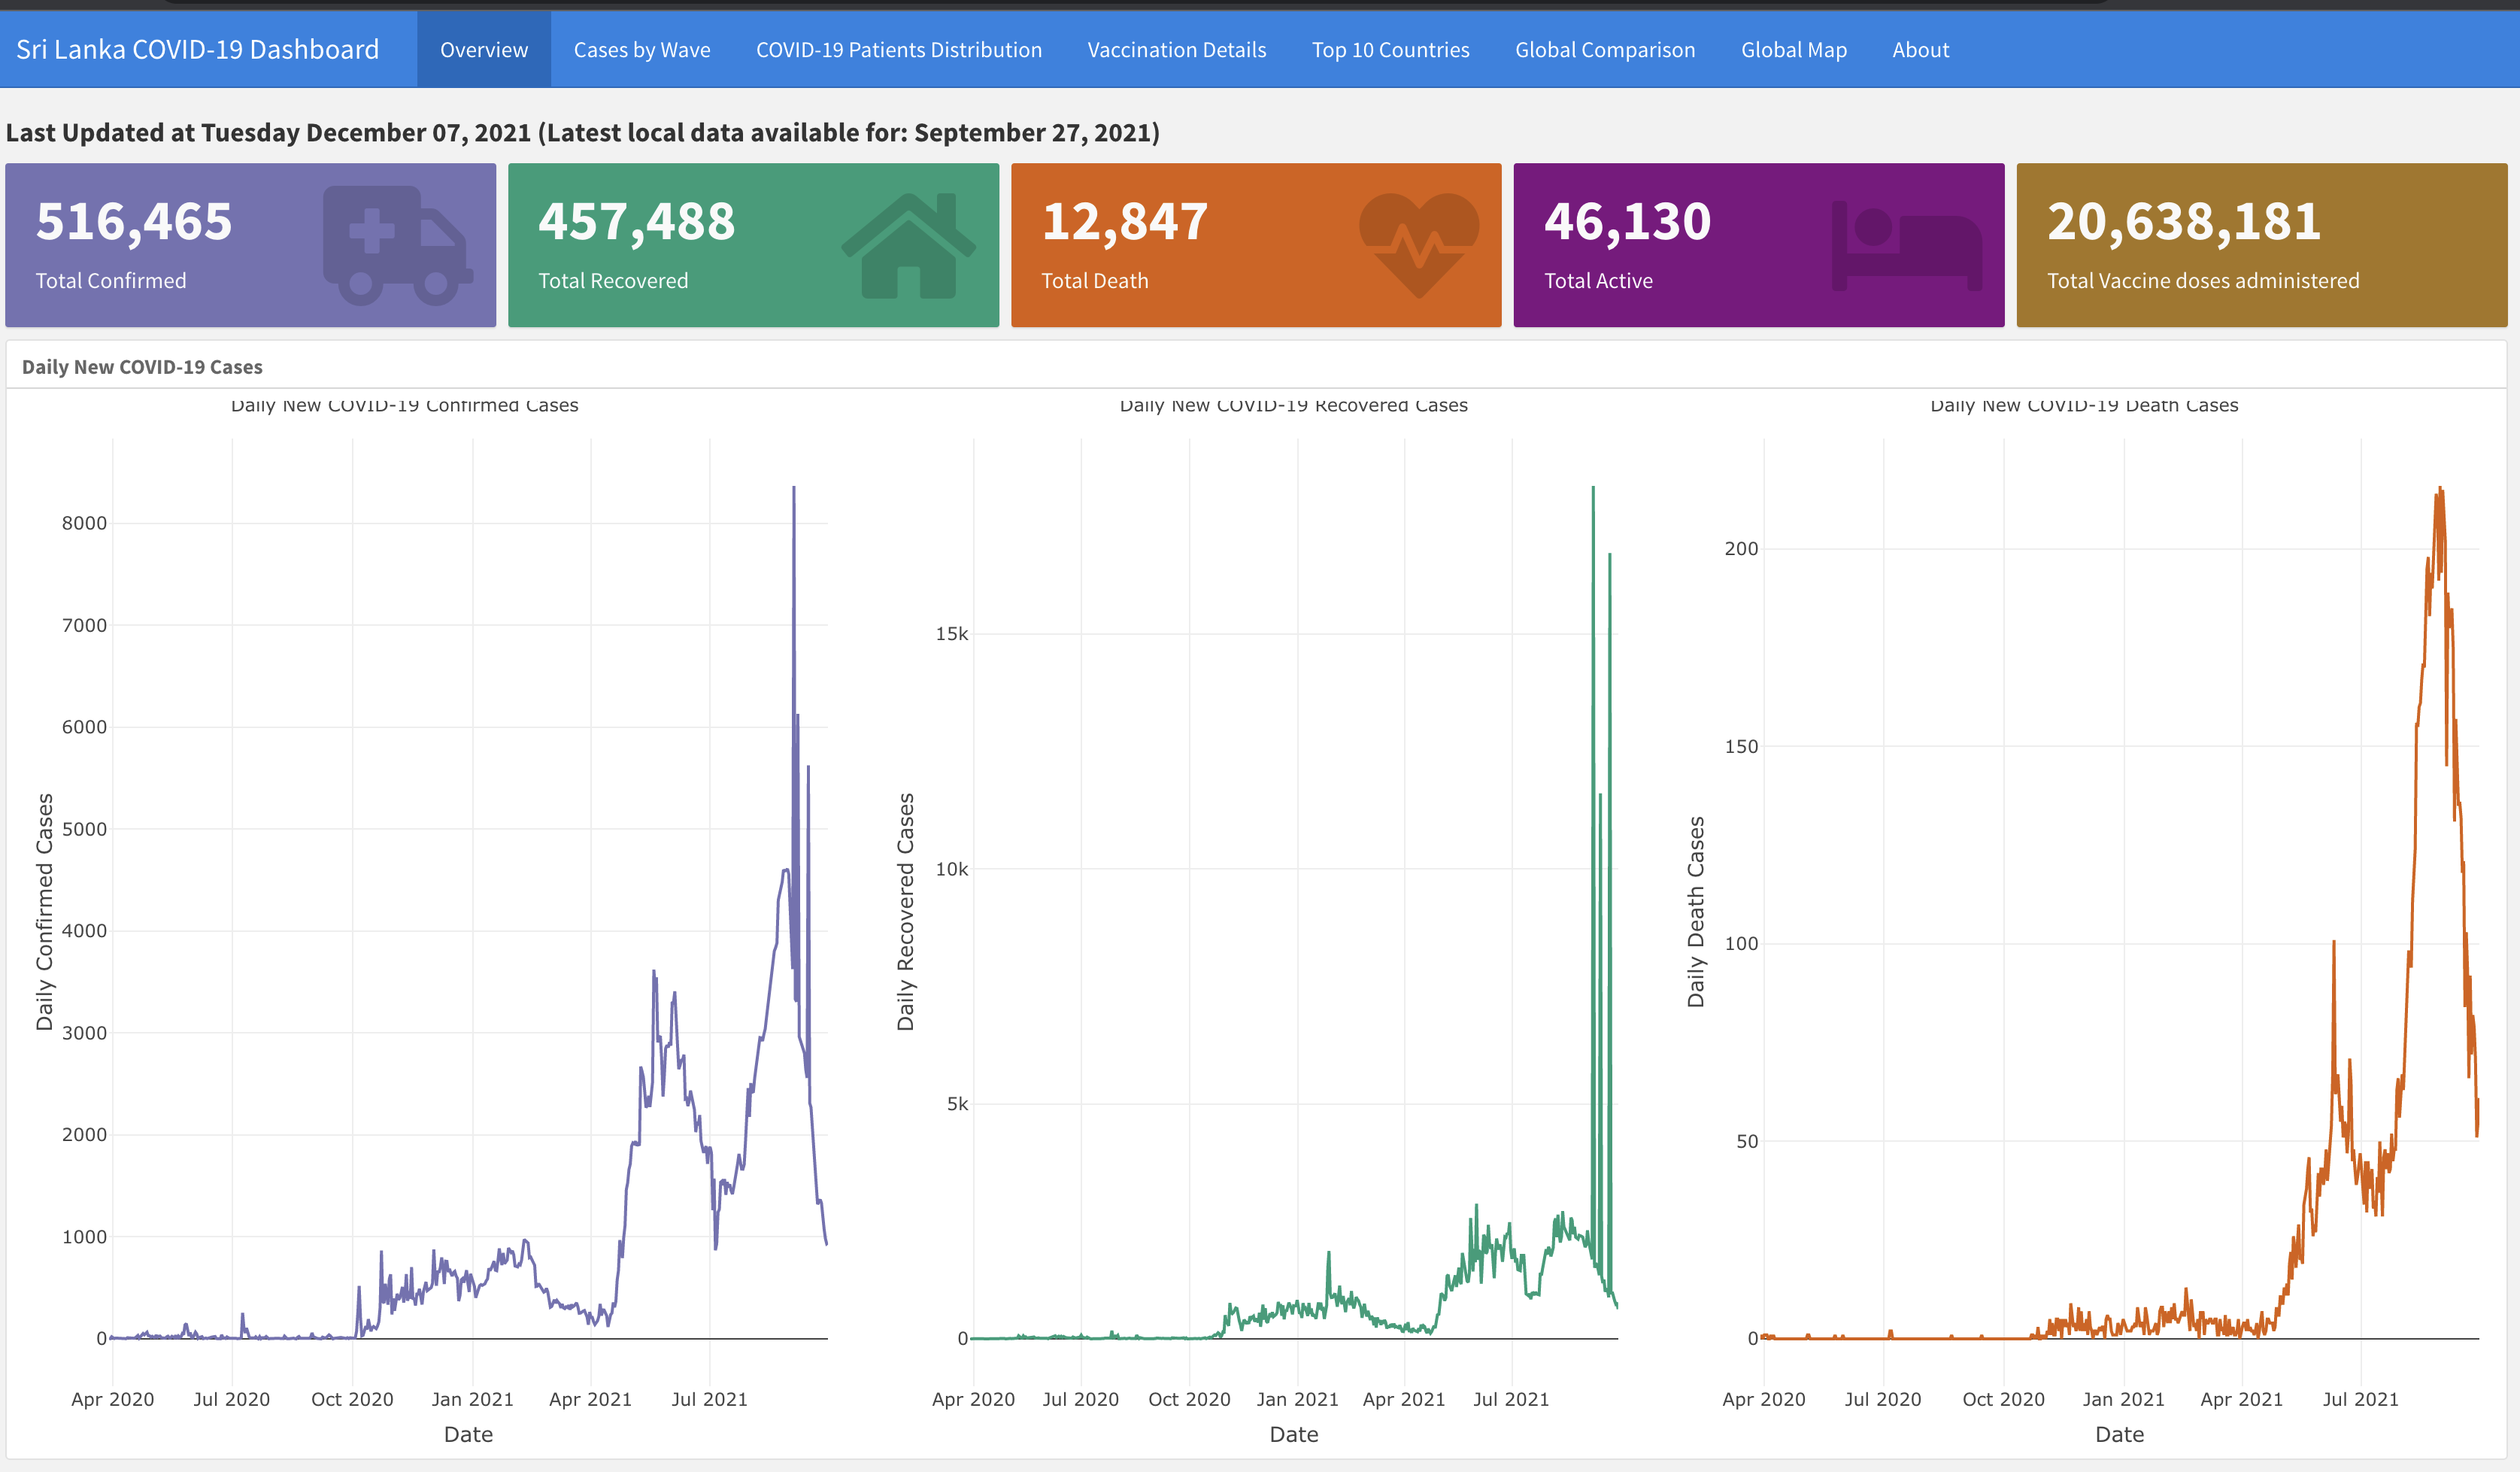
\includegraphics[width=0.8\linewidth]{images/dashboard} 

}

\caption{Overview Panel: Screeshot of the Dashboard}\label{fig:unnamed-chunk-1}
\end{figure}

\newpage

\textbf{Table 6: Description of the panels}

\begin{longtable}[]{@{}
  >{\raggedright\arraybackslash}p{(\columnwidth - 2\tabcolsep) * \real{0.13}}
  >{\raggedright\arraybackslash}p{(\columnwidth - 2\tabcolsep) * \real{0.87}}@{}}
\toprule
\textbf{Name of the Panel} & \textbf{Description of the Panel} \\
\midrule
\endhead
Overview & Total count of COVID-19 confirmed, recovered, deaths, active
cases \& total vaccine doses administered.\hfill\break Provide an
overview of daily COVID-19 confirmed, recovered \& deaths by
plots.\hfill\break \\
Cases by Wave & There are three tabs in this panel.\hfill\break  * Total
COVID-19 confirmed cases - Cumulative count of COVID-19 confirmed cases
with specific dates\hfill\break * COVID-19 Cases Distribution by Wave -
Daily confirmed cases by wave\hfill\break * COVID-19 Deaths Distribution
by Wave - Daily deaths by wave\hfill\break \\
COVID-19 Patients Distribution & Provide an overview of confirmed cases
district wise distribution. There are four tabs in this
panel.\hfill\break * Total COVID-19 Patients Distribution in Sri Lanka -
Total confirmed counts for each district is represented by tree
map\hfill\break * Country Map - Total confirmed cases in each district
represented by Sri Lanka country map\hfill\break * Distribution of Daily
COVID-19 Patients for Last 30 Days - Visualize the daily confirmed cases
distribution by districts in last 30 days\hfill\break * By Applying
Min-Max Transformation - Visualize the details in the third tab by
applying min-max transformation for each district\hfill\break \\
Vaccination Details & Provide an overview of COVID-19 vaccination in Sri
Lanka. There are two tabs.\hfill\break * Total Vaccine Doses - Visualize
the administered vaccine doses as first dose only \& fully
vaccinated\hfill\break * Total Administered Doses by Vaccine Name -
Visualize the vaccination by vaccine names\hfill\break \\
Top 10 Countries & In this panel, compare the Sri Lanka confirmed \&
deaths with top 10 countries in the world (top 10 countries - The
countries which have been reported highest number of confirmed cases as
31st of August 2021).\hfill\break There are two
tabs.\hfill\break * Comparison of Cumulative Cases in Sri Lanka with Top
10 Countries - Compare the confirmed and deaths in Sri Lanka with top 10
countries by cumulative time series plots\hfill\break * Comparison of
Log of Cumulative Cases in Sri Lanka with Top 10 Countries - Compare the
confirmed and deaths in Sri Lanka with top 10 countries by log
cumulative time series plots\hfill\break (The data has been pulled from
WHO)\hfill\break \\
Global Comparison & Compare the total confirmed \& deaths in Sri lanka
with top 10 countries in Global \& Asia. There are two
tabs.\hfill\break * Comparison of the sri Lanka with Top 10 Countries
Reporting the Most COVID-19 Cases in the World - Compare the total
confirmed \& deaths in Sri Lanka with top 10 countries in the world \&
compare the case fatality ratios\hfill\break * Comparison of the sri
Lanka with Top 10 Countries Reporting the Most COVID-19 Cases in the
Asia - Compare the total confirmed \& deaths in Sri Lanka with top 10
countries in the Asia \& compare the case fatality ratios\hfill\break \\
Global Map & Visualize the distribution of confirmed, recovered \&
deaths in the world by world map.\hfill\break \\
About & This panel contains the details about the dashboard. \\
\bottomrule
\end{longtable}

\begin{figure}
\centering
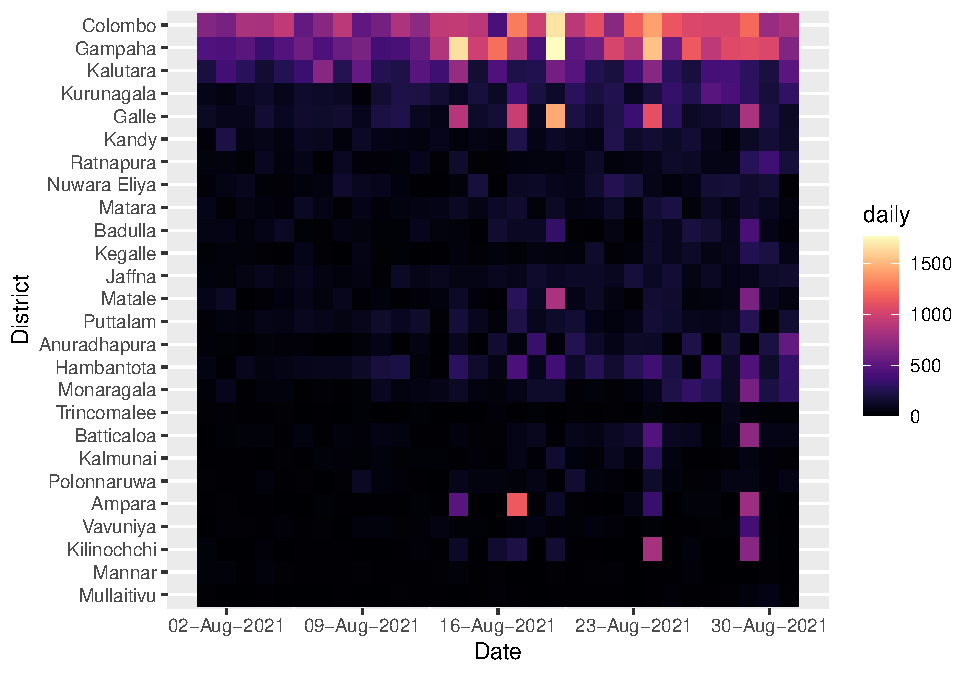
\includegraphics{manuscript_covid19dashboard_files/figure-latex/unnamed-chunk-3-1.pdf}
\caption{Distribution of COVID19 Cases by Districts: (A) Plotted on a
Single Panel, (B) Plotted on Separate Panels.}
\end{figure}

\begin{figure}
\centering
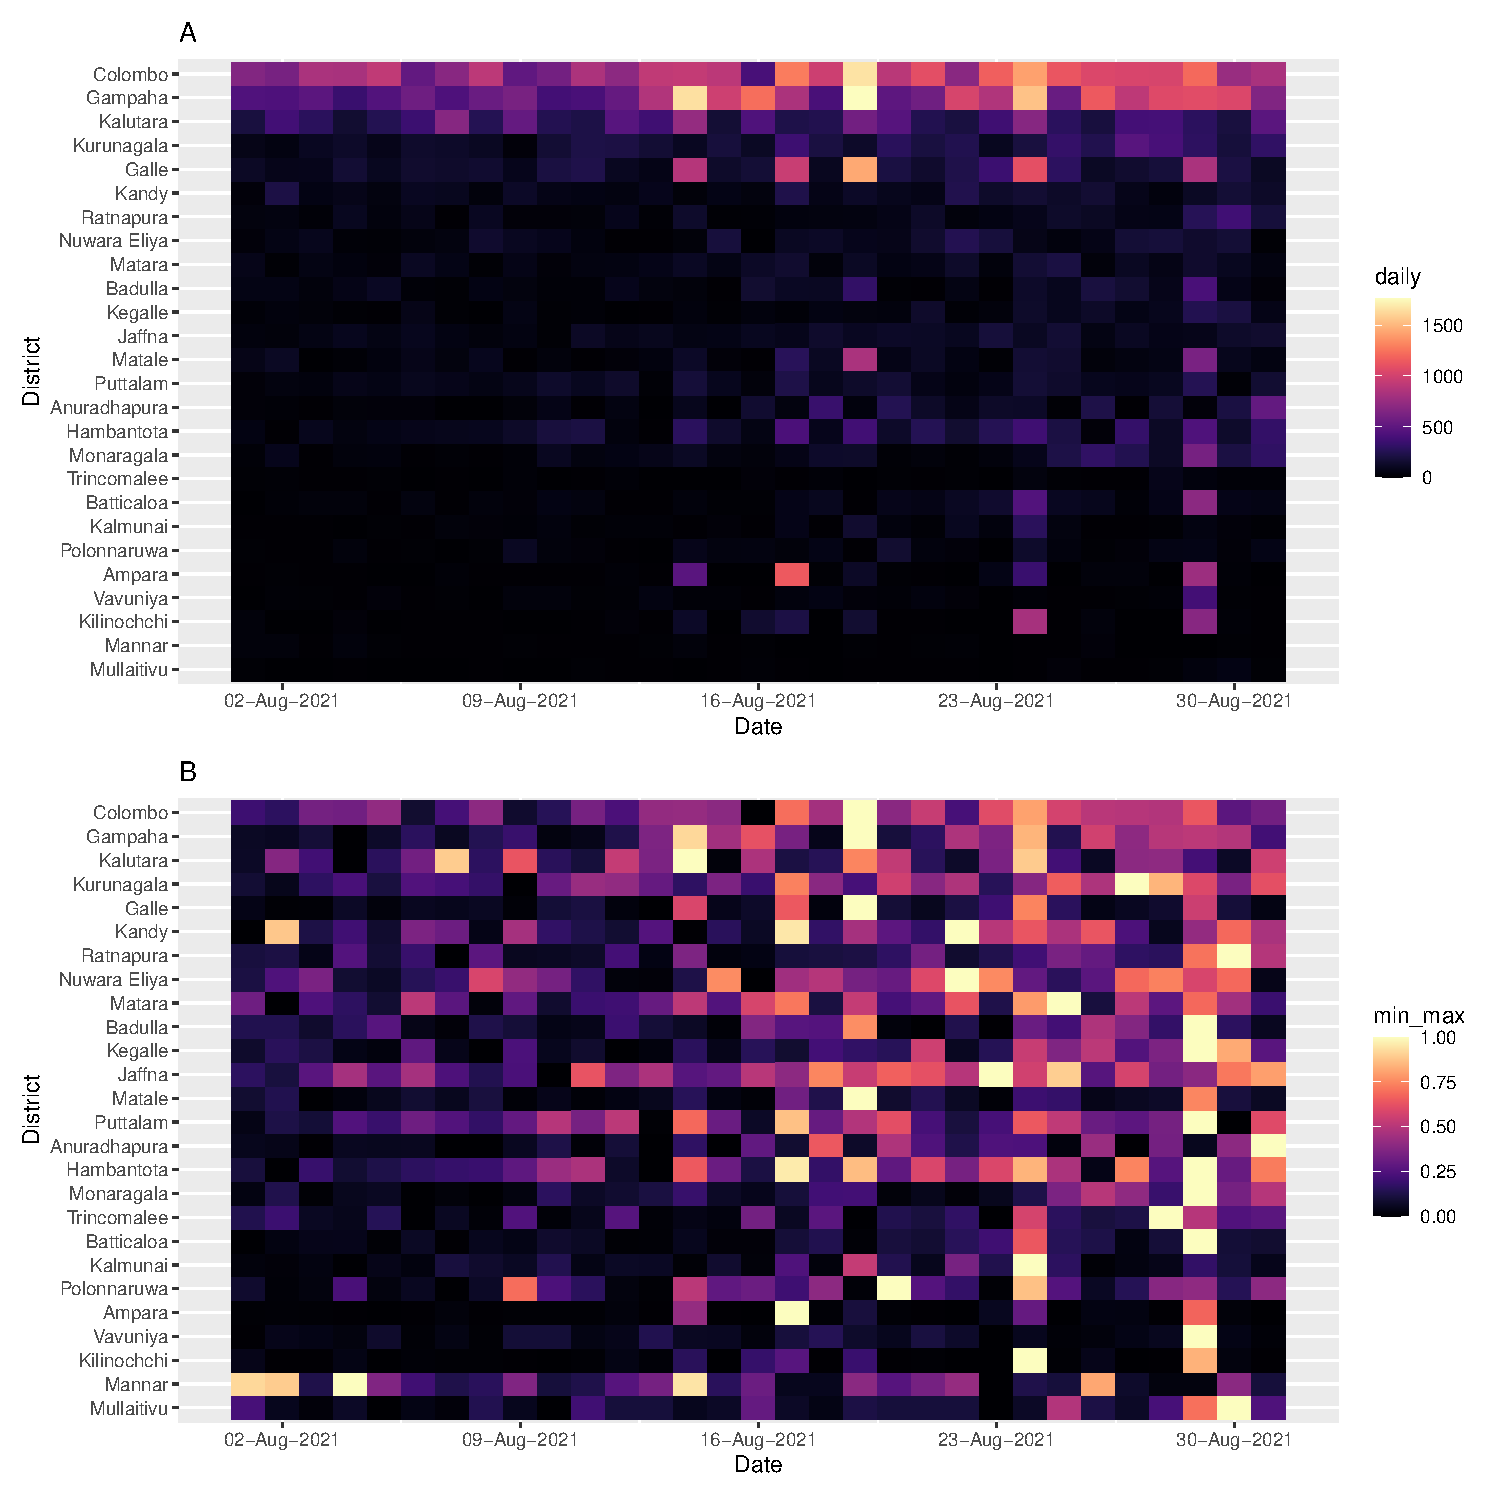
\includegraphics{manuscript_covid19dashboard_files/figure-latex/unnamed-chunk-4-1.pdf}
\caption{(A) Global View of Distribution of COVID19 Cases by DIstricts,
(B) Local View of Distribution of COVID19 Cases by Districts}
\end{figure}

We now describe the novel visualization approaches we included in out
dashboard. To effectively distribute the vaccine and to support
situational awareness and inform policy makers decision making it is
important to know the district-wise spread of COVID-19 cases. We have
daily COVID-19 data related to confirmed cases in all 25 districts in
Sri Lanka. This structure generates a multiple time series collection.
Visualizing these time series data is useful to identify similarities
and dissimilarities between districts and their general trends. There
are two approaches to visualizing these time series: (i) drawing
individual time series plots for each district (as shown in Figure 2),
and (ii) simultaneously plots all time series on a single panel (as
shown in Figure 3). Plotting all time series simultaneously is also not
possible due to overlapping time series and scale differences. Plotting
separate panels for each district is not effective. The reason is that
it is hard to compare across 25 different panels at once. In order to
overcome these problems in multiple time series visualization, we use
heat maps ((Peng (2008))) to visualize global and local similarities and
dissimilarities across districts. The associated results are shown in
Figure 3. Here two heatmaps are used to show the global variations
(Figure 3: A) and local variation (Figure 3: B) in the time series
collection. Figure 3-A cell colours represent the actual counts of the
COVID-19 confirmed cases. This is useful to get an idea about the
differences in absolute values. Figure 3-B cell colours represent the
normalized values created applying the min-max transformation. Min-max
transformation is applied to each district time series by using the
corresponding district minimum and maximum value of the time series.
This helps us to get an idea about patterns within districts. For
example, according to Figure 3A we can see Colombo, Gampaha and Kalutara
districs COVID-19 cases are significantly higher than other districts.
According to Figure 3B all districts show an increasing trend pattern as
the right-hand side of the cells are lighter than the left-hand side
cells in the heat map. Furthermore according to Figure 3B all districts
reported high number of cases on 19, 24, 29 August, 2021. Figure 3B is
useful for identifying these local outlying behaviours. As shown in
Figure 4, we also use Choropleth map and Dorling cartogram to visualize
spatial distribution of COVID-19 cases. The vaccination information are
visualize through interactive time series plots and bar charts. A
screenshot of associated panels are shown in Figure 5 and Figure 6.

\begin{figure}
\centering
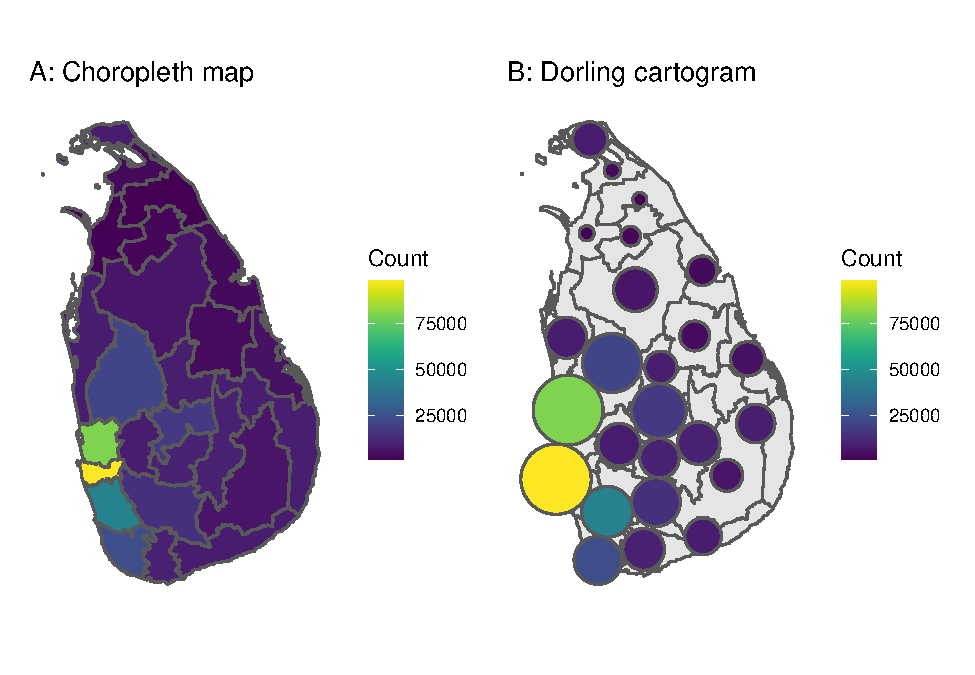
\includegraphics{manuscript_covid19dashboard_files/figure-latex/unnamed-chunk-5-1.pdf}
\caption{Spatial DIstribution of COVID1-19 Cases by Districts}
\end{figure}

\begin{figure}

{\centering 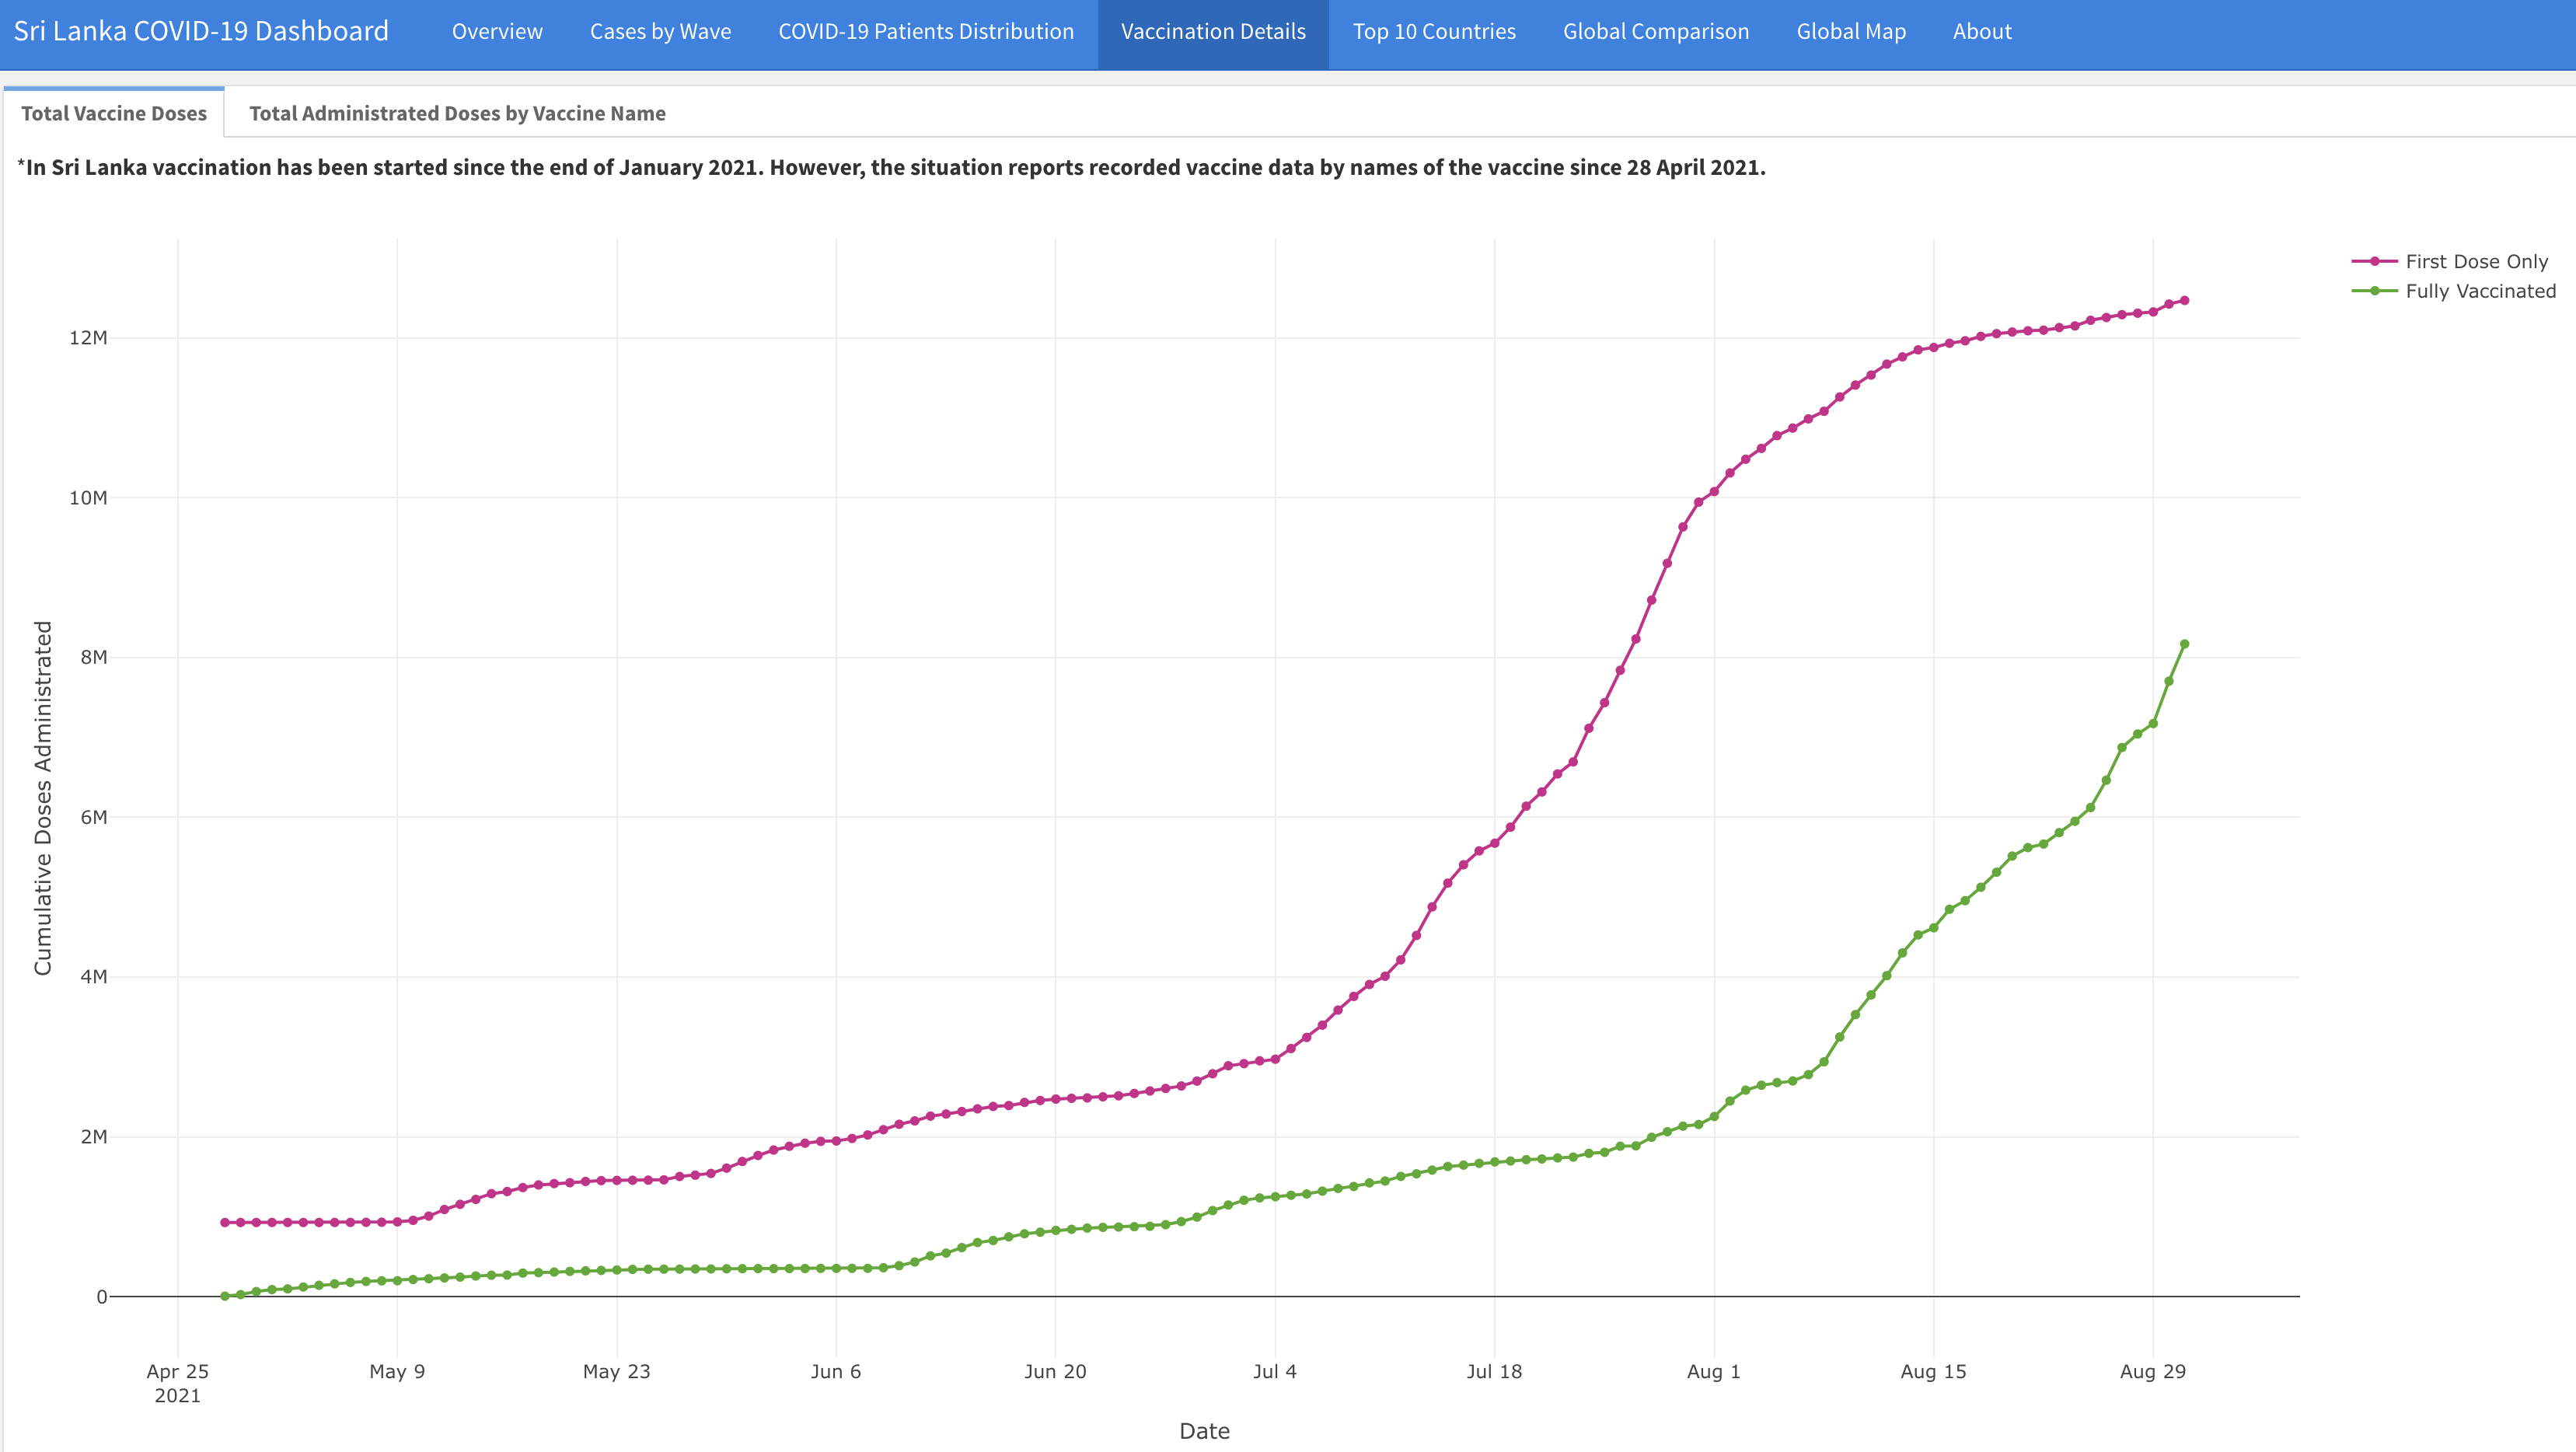
\includegraphics[width=0.8\linewidth]{Images/d3} 

}

\caption{Time Series Plot of Distribution of First Dose and Second Dose}\label{fig:unnamed-chunk-6}
\end{figure}

\begin{figure}

{\centering 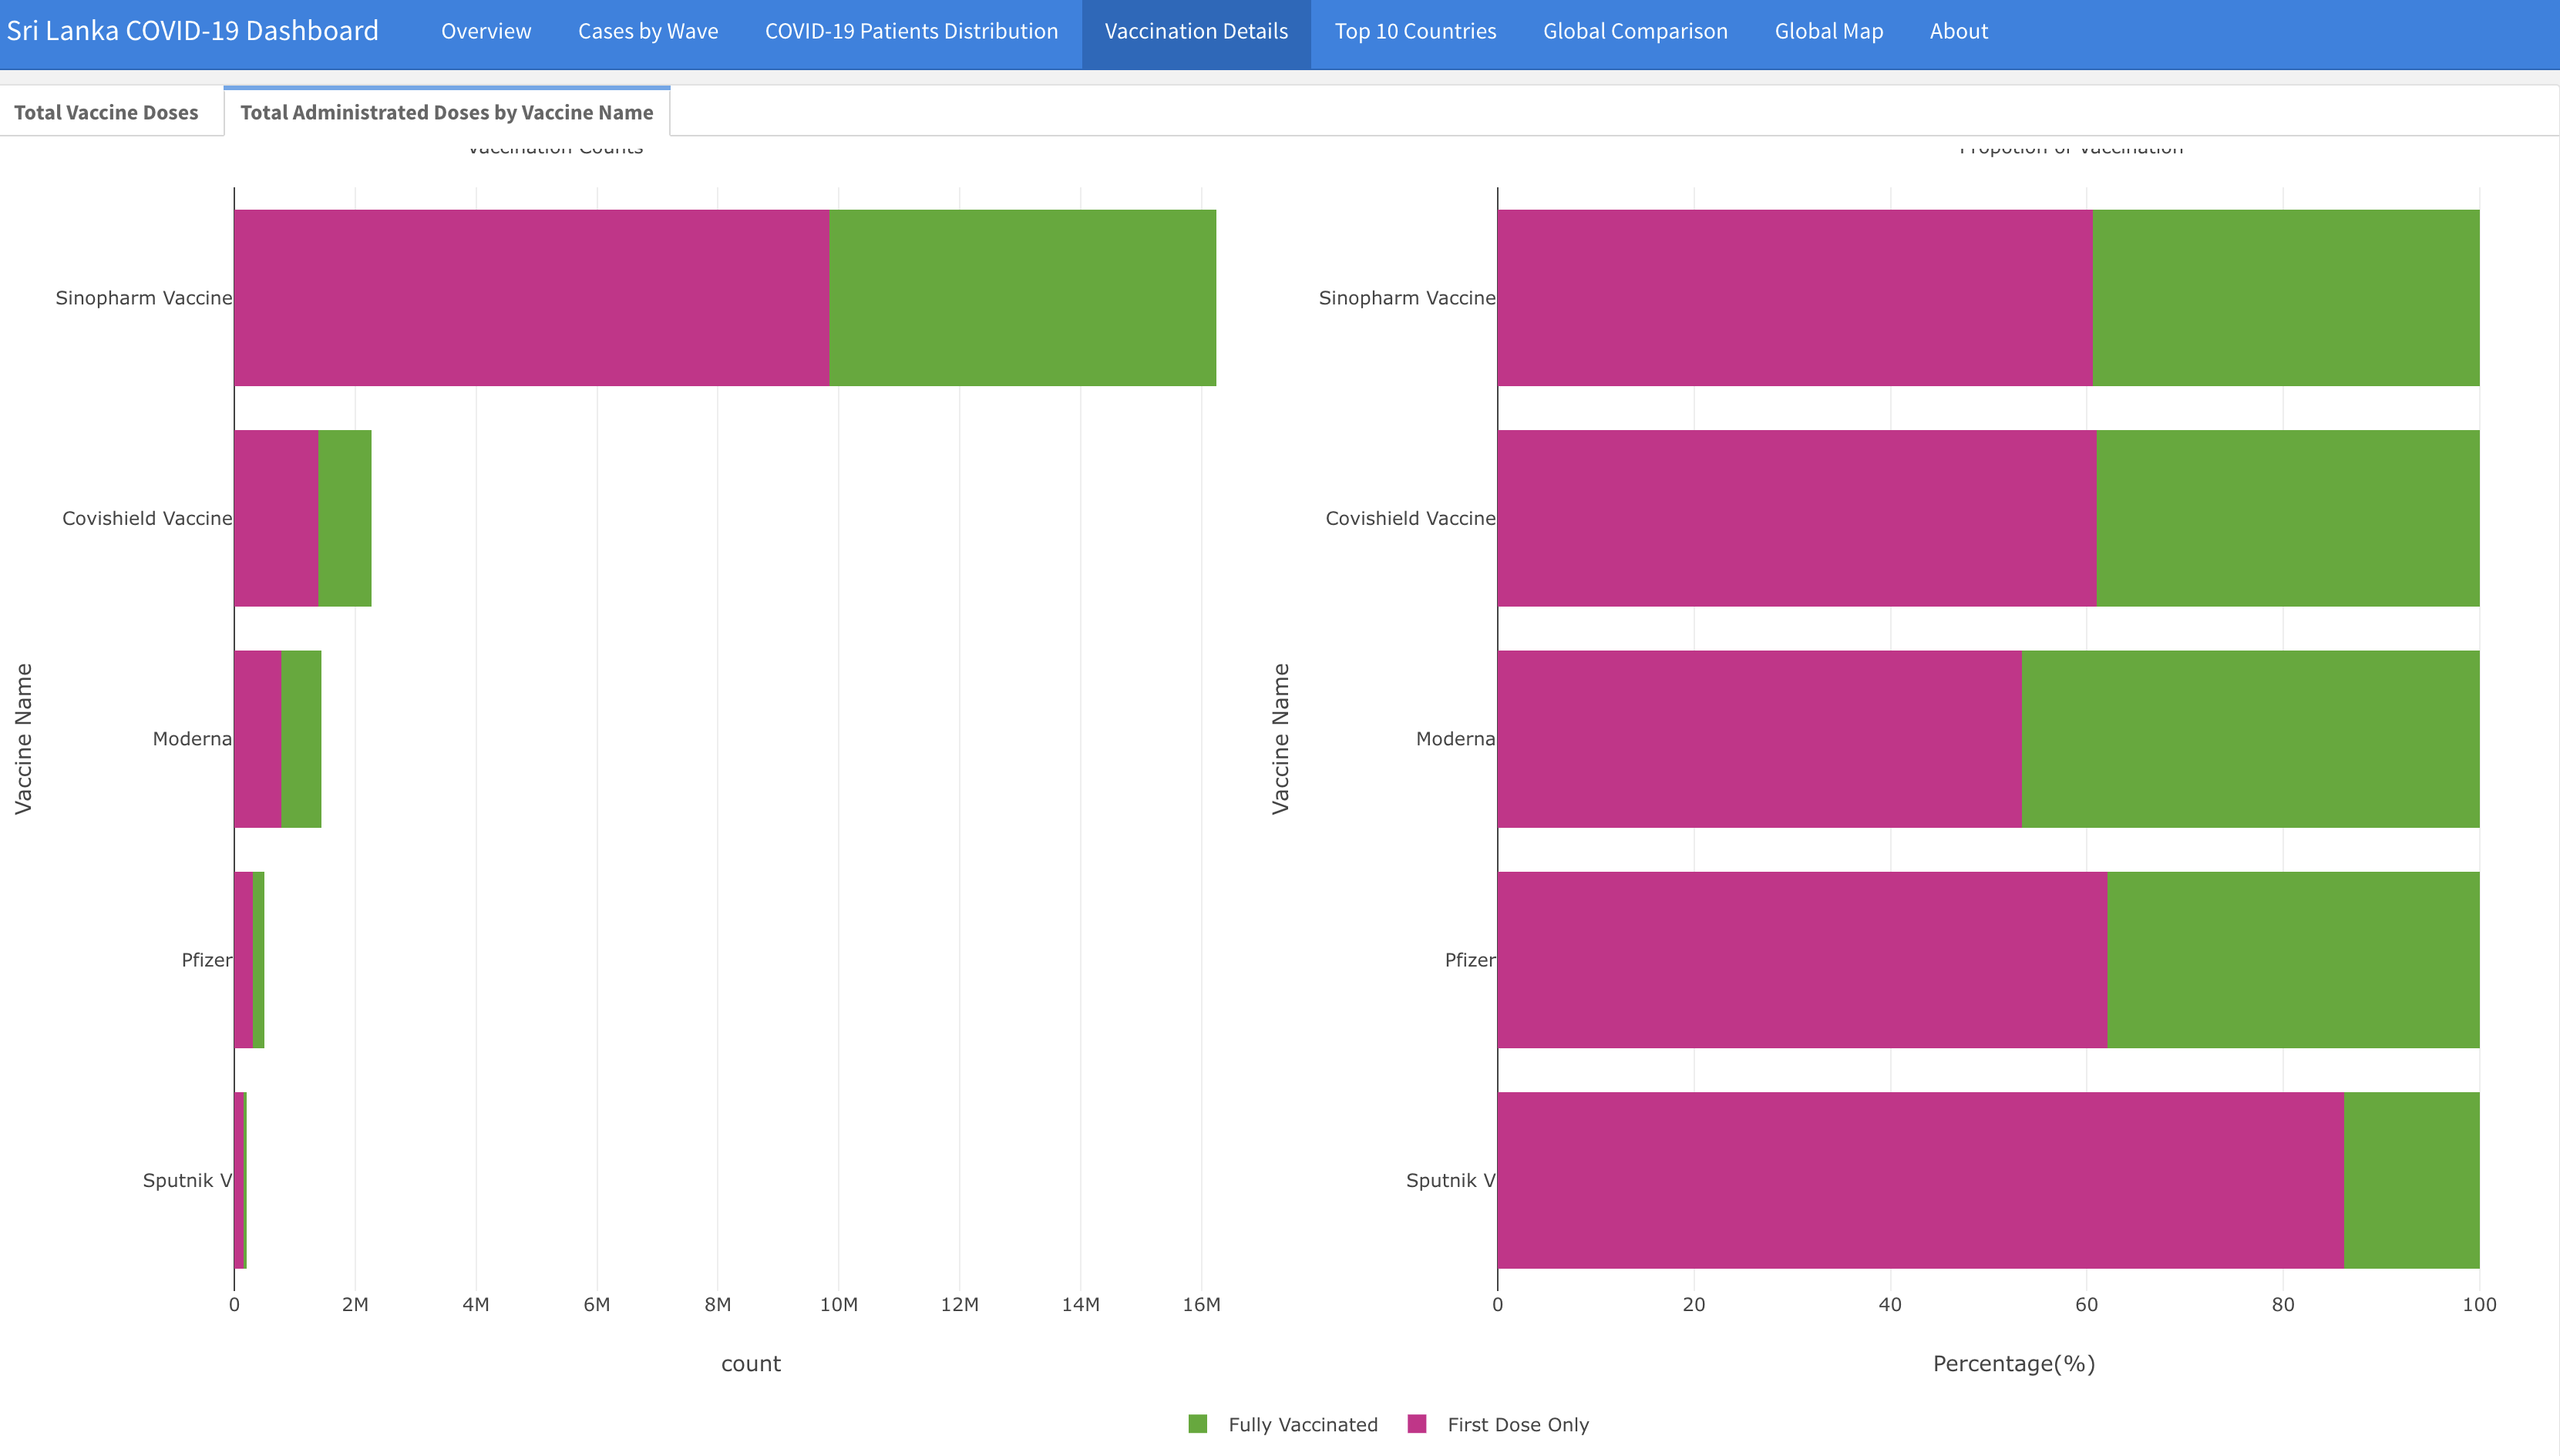
\includegraphics[width=0.8\linewidth]{Images/d2} 

}

\caption{Distribution of Vaccines by Different Types and Dose}\label{fig:unnamed-chunk-7}
\end{figure}

\hypertarget{conclusions}{%
\section{Discussion and Further research}\label{conclusions}}

Bar charts and line charts are the most frequently used tools for the
visualization of total cases, daily cases and comparisons with respect
to time. Some dashboards contained doughnut shape pie charts to
summarize the total figures. In almost each and every dashboard, value
boxes have been used to represent total figures. Some dashboards
contained interactive maps \& data tables to visualize the distribution
of cases by country, province, region or state. All dashboards are daily
updating real time dashboards. Gender, age groups and ethnicity can be
identified as common breakdowns. The data sets \& related links are
available on most of the dashboards \& can be downloaded. It can be seen
that it is very easy, clear and user friendly to identify confirmed,
recovered and deceased cases in dashboards which include one color theme
for the whole dashboard. Dashboards with the dark background are more
comfortable to the eyes than dashboards with light background \& light
colors. Also, it is better if the dashboard can be fitted on a single
screen rather than adjusting through a grid overlay.

\hypertarget{references}{%
\section{References}\label{references}}

\hypertarget{refs}{}
\begin{CSLReferences}{1}{0}
\leavevmode\hypertarget{ref-belgium}{}%
{``{COVID 19 Dashboard -- Belgium}.''} 2022.
\url{https://esribelux.maps.arcgis.com/apps/ops\%0Adashboard/index.html\#/e350724c87af49bb9ce29646f8a42344}.

\leavevmode\hypertarget{ref-indiadash}{}%
{``{COVID 19 Dashboard India -- ZOHO Analytics -- ZOHO}.''} 2022.
\url{https://www.zoho.com/covid/india/}.

\leavevmode\hypertarget{ref-nhs}{}%
{``{COVID 19 Dashboard -- NHS providers}.''} 2022.
\url{https://nhsproviders.org/topics/covid-\%0A19/tracking-covid-19-data/covid-19-dashboard}.

\leavevmode\hypertarget{ref-italy}{}%
{``{COVID-19 integrated surveillance data in Italy -- EpiCentro}.''}
2022.
\url{https://www.ep\%0Aicentro.iss.it/en/coronavirus/sars-cov-2-dashboard}.

\leavevmode\hypertarget{ref-jamaica}{}%
{``{COVID-19 Jamaica - Ministry of Health and Wellness}.''} 2021.
\url{https://jamcovid19.moh.gov.jm/}.

\leavevmode\hypertarget{ref-sl}{}%
{``{COVID-19: Live situational Analysis Dashboard of Sri Lanka}.''}
2022. \url{https:\%0A//hpb.health.gov.lk/covid19-dashboard/}.

\leavevmode\hypertarget{ref-jh}{}%
{``{COVID-19 Map -- Johns Hopkins Coronavirus Resource Center}.''} 2022.
\url{https://coronavi\%0Arus.jhu.edu/map.html}.

\leavevmode\hypertarget{ref-nssac}{}%
{``{COVID-19 Surveillance Dashboard -- NSSAC Research}.''} 2022.
\url{https://nssac.bii.virg\%0Ainia.edu/covid-19/dashboard/}.

\leavevmode\hypertarget{ref-za}{}%
{``{COVID-19 ZA Dashboard - Data Studio}.''} 2021.
\url{https://datastudio.google.com/u/0/\%0Areporting/1b60bdc7-bec7-44c9-ba29-be0e043d8534/page/hrUIB}.

\leavevmode\hypertarget{ref-flexdashboard}{}%
Iannone, Richard, JJ Allaire, and Barbara Borges. 2020.
\emph{Flexdashboard: R Markdown Format for Flexible Dashboards}.
\url{https://CRAN.R-project.org/package=flexdashboard}.

\leavevmode\hypertarget{ref-rami}{}%
Krispin, Rami. 2021. {``{The Coronavirus Dashboard}.''}
\url{https://github.com/RamiKrispin/coronavirus_dashboard}.

\leavevmode\hypertarget{ref-nz}{}%
{``{New Zealand COVID-19 Surveillance Dashboard}.''} 2021.
\url{https://nzcoviddashboard.esr.c\%0Ari.nz/\#!/}.

\leavevmode\hypertarget{ref-pakistan}{}%
{``{Pakistan's Official COVID-19 Dashboard -- Shifa International
Hospitals Ltd}.''} 2021.
\url{https://www.shifa.com.pk/covid-19-pakistan/}.

\leavevmode\hypertarget{ref-peng2008method}{}%
Peng, Roger D. 2008. {``A Method for Visualizing Multivariate Time
Series Data.''}

\leavevmode\hypertarget{ref-rki}{}%
{``{RKI COVID-19 Germany -- ArcGIS Experience}.''} 2021.
\url{https://experience.arcgis.co\%0Am/experience/478220a4c454480e823b17327b2bf1d4}.

\leavevmode\hypertarget{ref-plotly}{}%
Sievert, Carson. 2020. \emph{Interactive Web-Based Data Visualization
with r, Plotly, and Shiny}. Chapman; Hall/CRC.
\url{https://plotly-r.com}.

\leavevmode\hypertarget{ref-talagala}{}%
Talagala, Thiyanga S. 2021. \emph{Covid19srilanka: The 2019 Novel
Coronavirus COVID-19 (2019-nCoV) Data in Sri Lanka}.
\url{https://github.com/thiyangt/covid19srilanka}.

\leavevmode\hypertarget{ref-russia}{}%
{``{The Global COVId-19 Index (GCI) -- Russia Dashboard -- PEMANDU
Associates}.''} 2021. \url{https://covid19.pemandu.org/Russia}.

\leavevmode\hypertarget{ref-canada}{}%
{``{Track COVID-19 Across Canada Using Our Interactive Dashboards}.''}
2021.
\url{https:\%0A//samples.dundas.com/Dashboard/62cef916-5488-4d3b-9c57-204092d01813?e=false\&vo=viewonly}.

\leavevmode\hypertarget{ref-who}{}%
{``{WHO Coronavirus (COVID-19) Dashboard}.''} 2021.
\url{https://covid19.who.int/region/amro/country/us}.

\end{CSLReferences}

\newpage

\hypertarget{appendix-overview-of-reviewed-dashboard}{%
\section{Appendix: Overview of reviewed
dashboard}\label{appendix-overview-of-reviewed-dashboard}}

Real time updated COVID-19 dashboard created by the John Hopkins
University Center for Systems Science \& Engineering (JHU CSSE) has
included total confirmed cases \& total deaths by country,
province/region/state (not for all countries){[}6{]}. Weekly \& daily
global confirmed cases, deaths \& vaccine doses have been visualized
using bar plots related to the date in the side panels. Also, an
interactive world map has included in the dashboard to represent total
confirmed cases, incidence rate, fatality ratio \& vaccine doses
administered by country \& state of US. All the links related to the
data sets has been included in the dashboard. In this dashboard red,
white, green colors has been used to indicate confirmed cases, deaths \&
vaccine doses respectively. The dashboard has fitted on a single screen.

\begin{figure}
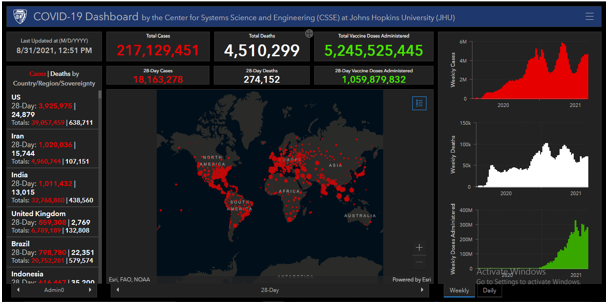
\includegraphics[width=8.42in]{Images/1} \caption{Johns Hopkins University COVID-19 Dashboard}\label{fig:unnamed-chunk-8}
\end{figure}

Live updated ``WHO COVID-19 dashboard'' contained four panels. The
interactive world map in the dashboard has visualized the distribution
of COVID-19 confirmed cases, deaths \& vaccination by country {[}15{]}.
Line chart \& bar charts have been used as visualization plots. Blue,
red, green colors have been used to represent confirmed cases, deaths \&
vaccination respectively. The links related to the underlying data was
available in the dashboard. The dashboard was not fitted on a single
screen.

\begin{figure}
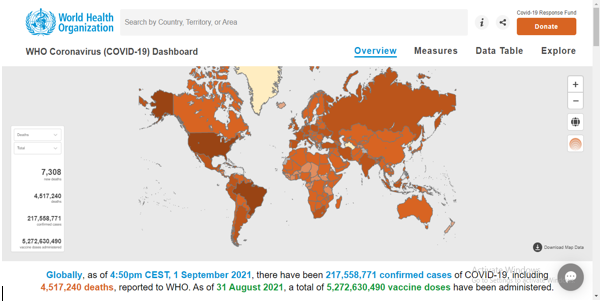
\includegraphics[width=8.35in]{Images/2} \caption{WHO COVID-19 Dashboard}\label{fig:unnamed-chunk-9}
\end{figure}

The ``COVID-19 surveillance dashboard'' created by the University of
Virginia in collaboration with Bio complexity Institute has included
interactive world map with a time slide to visualize the confirmed
cases, recovered cases, deaths, active cases \& vaccine details {[}7{]}.
Line charts, bar charts \& data tables have been visualized in the
dashboard. Red, blue, green \& yellow colors have been used to identify
confirmed, deceased, recovered \& active cases respectively. The data
behind the dashboard also available on the dashboard \& can be
downloaded. The dashboard has fitted on a single screen.

\begin{figure}
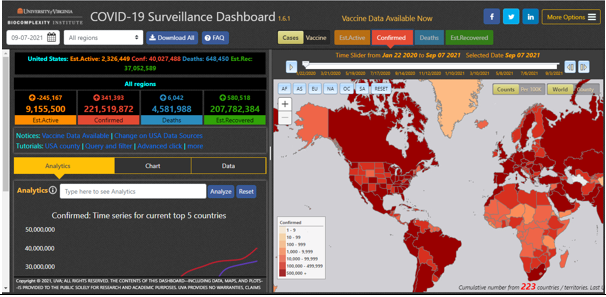
\includegraphics[width=8.42in]{Images/3} \caption{COVID-19 Surveillance Dashboard}\label{fig:unnamed-chunk-10}
\end{figure}

Corona cases (COVID-19) per municipality in Belgium dashboard has
included interactive map for distribution of total confirmed cases per
municipality, bar chart for number of cases per province, line charts
for number of cases per day by region \& municipality, dodge bar chart
for deaths per region, per age \& pie chart for deaths per age as
visualization methods{[}3{]}. Also it included several value boxes for
total cases, total deaths \& hospital situations. There was no specific
color theme used in this dashboard. This dashboard also fitted on a
single screen.

\begin{figure}
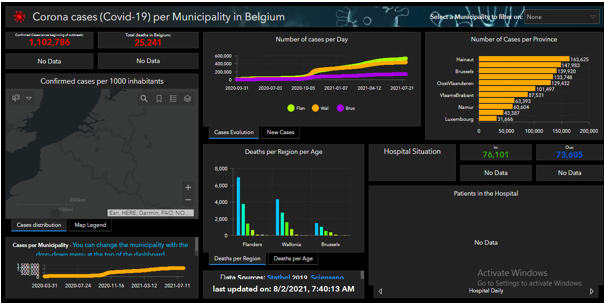
\includegraphics[width=8.39in]{Images/4} \caption{Corona cases per Municipality in Belgium Dashboard}\label{fig:unnamed-chunk-11}
\end{figure}

The COVID-19 dashboard for England created by NHS providers included
daily totals, daily changes \& weekly changes in new cases, hospital
admission, patients in hospital, and patients in ICU beds, deaths \&
vaccinations in England as counts {[}2{]}. Bar plots for daily new
cases, hospital admissions \& deaths for last 30 days have been added in
this dashboard. Also it has included data table for total count, daily
changes (as increase or decrease), weekly changes (as increase or
decrease) of new cases \& hospital admission by region. It can be seen
that, three different colors have been used in bar plot as orange for
new cases, green for hospital admissions \& red for deaths. These plots
were not interactive plots \& there was only one panel. The dashboard
was not fitted on a single screen.

\begin{figure}
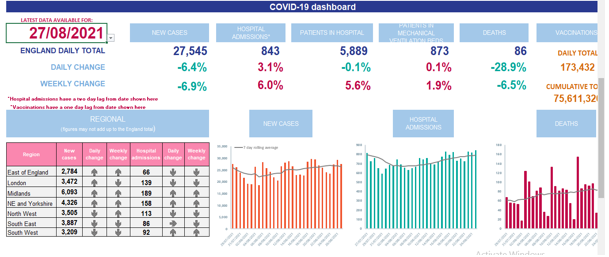
\includegraphics[width=8.46in]{Images/5} \caption{COVID-19 dashboard for England}\label{fig:unnamed-chunk-12}
\end{figure}

The Environmental Science and Research Institute COVID-19 dashboard for
New Zealand (was developed \& is maintained in collaboration with
Epi-interactive Ltd) contained five panels as overview, outbreak,
source, international \& ESR reports {[}10{]}. In this real time updated
dashboard, they have included value boxes for total confirmed cases,
recovered cases, deaths \& interactive map has been added for
distribution of confirmed \& probable cases as incidence \& count. Also
they have included bar charts for confirmed cases distribution by
gender, age group, \& line charts for confirmed \& deaths as daily \&
cumulative. The dashboard has not fitted on a single screen.

\begin{figure}
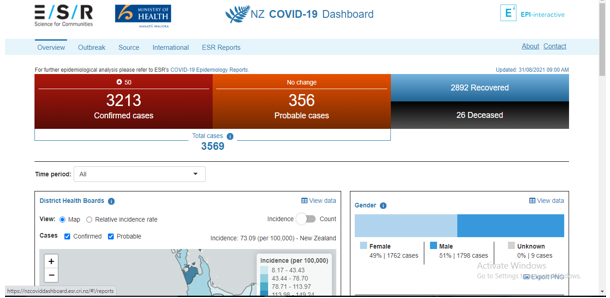
\includegraphics[width=8.47in]{Images/6} \caption{New Zealand COVID-19 Dashboard}\label{fig:unnamed-chunk-13}
\end{figure}

Pakistan's official COVID-19 dashboard is a real time updated dashboard
with one panel. This dashboard contains value boxes for total confirmed
cases, active cases, deaths, recovered cases by country. Province wise
cases have been represented by map \& data table {[}11{]}. Line charts
\& bar charts have been added to visualize the distribution of cases
related to time \& province. In the value boxes blue, orange, pink \&
green colors have been applied for confirmed cases, active cases, deaths
\& recoveries respectively, but there was no specific color theme used
when plotting the graphs. The dashboard cannot be seen on a single
screen without grid overlay.

\begin{figure}
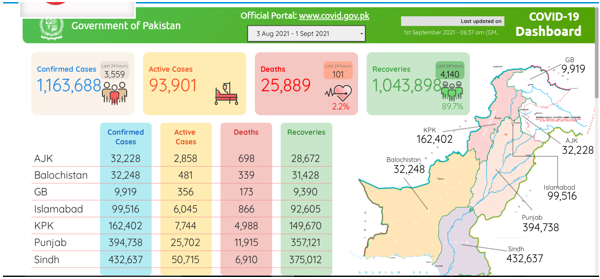
\includegraphics[width=8.33in]{Images/7} \caption{COVID-19 Dashboard for Pakistan}\label{fig:unnamed-chunk-14}
\end{figure}

COVID-19 Canada live dashboard has been developed with three panels for
provincial data, hospital resources \& projections {[}14{]}. This
dashboard contained interactive map for represented total reported cases
\& deaths by province. Data tables, line charts, bar charts were the
most frequently used visualization types of this dashboard. More details
were presented on this dashboard by province like ventilator counts,
hospital beds per 100 residents, resource capacity based on critical
case rate, effect of social distance, forecast of deaths \& cases. There
was no specific color theme applied for plotting the graphs. The
dashboard also was not fitted on a single screen.

\begin{figure}
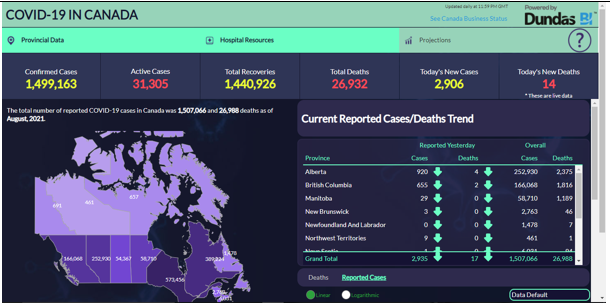
\includegraphics[width=8.47in]{Images/8} \caption{COVID-19 in Canada dashboard}\label{fig:unnamed-chunk-15}
\end{figure}

``Zoho analytics COVID-19 live dashboard'' for India contained three
panels as insight by state, trend analysis \& vaccination {[}1{]}.
Interactive country map has been used to visualize the distribution of
confirmed cases, active cases, deaths, recovered cases \& vaccination by
states in India. Line charts, bar charts \& doughnut shape pie charts
have been used as other visualization tools. Also this dashboard
contained data table for overview of COVID-19 in India. This dashboard
also was not fitted on a single screen.

\begin{figure}
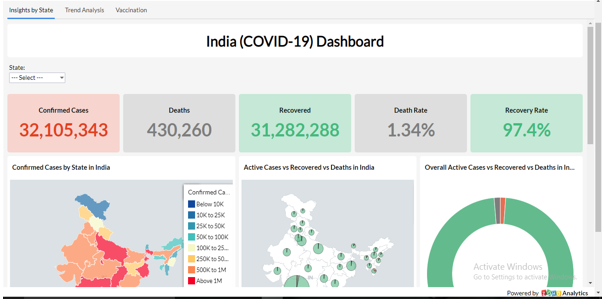
\includegraphics[width=8.42in]{Images/9} \caption{India COVID-19 Dashboard}\label{fig:unnamed-chunk-16}
\end{figure}

Italy COVID-19 dashboard created by the COVID-19 task force of the
department of infection diseases and the IT service Istituto Superiore
Sanita, contained interactive map, bar charts, doughnut shape pie charts
\& heat maps as visualization tools {[}4{]}. It provides data related to
COVID-19 cases, cases distribution by age, clinical status, and weekly
number of cases notified in Italy by region/province. This dashboard
also was not fitted on a single screen.

\begin{figure}
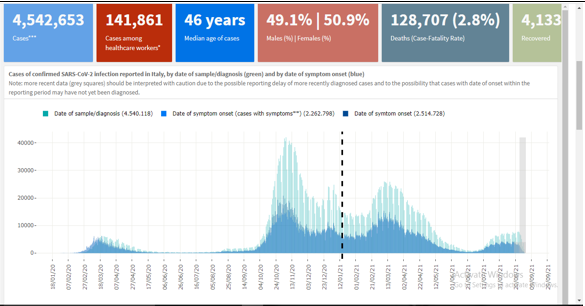
\includegraphics[width=8.12in]{Images/10} \caption{Italy COVID-19 Dashboard}\label{fig:unnamed-chunk-17}
\end{figure}

Live COVID-19 dashboard developed \& contributed by an amber innovations
for the government of Jamaica has added interactive country map \& data
table to represent the COVID- 19 cases by parish {[}9{]}. Line charts \&
bar charts have been added to the dashboard for cumulative \& daily
COVID-19 cases. Yellow, green \& red colors have been used to represent
confirmed, recovered \& deaths respectively. Doughnut shape pie chart
has been added to represent the distribution of recovered, confirmed \&
deaths by age group. This dashboard was not fitted on a single screen.

\begin{figure}
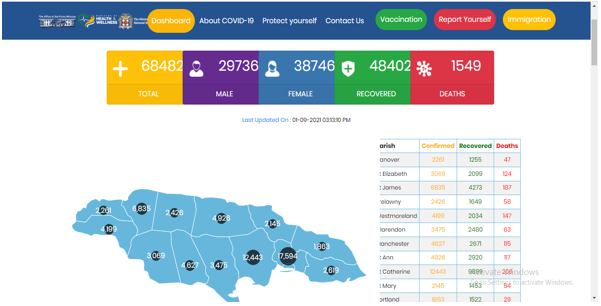
\includegraphics[width=8.35in]{Images/11} \caption{Jamaica COVID-19 Dashboard}\label{fig:unnamed-chunk-18}
\end{figure}

The GCI COVID-19 dashboard for Russia includes an interactive map, bar
charts \& line charts to visualize the COVID-19 data {[}13{]}. Yellow,
green, red \& blue colors have been added to identify the confirmed,
recovered, deaths \& active case respectively in plotting the charts.

\begin{figure}
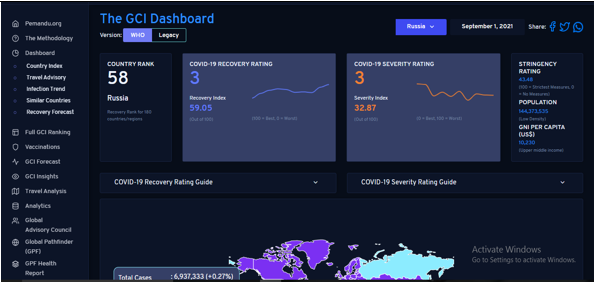
\includegraphics[width=8.25in]{Images/12} \caption{GCI COVID-19 Dashboard for Russia}\label{fig:unnamed-chunk-19}
\end{figure}

COVID-19 live situation analysis dashboard of Sri Lanka contains total
\& daily figures in Sri Lanka as counts {[}5{]}. Total cases \& active
cases have been visualized by using a line chart. Bar charts have been
used to summarize the daily confirmed cases and recovered cases. As well
fatality rate, recovery rate \& daily investigations using PCR tests \&
rapid antigen tests have been compared by using the bar charts. Doughnut
shape pie chart has been used to summarize the total cases. Blue, green
\& red colors have been applied to active, recovered \& deaths
respectively. This dashboard was also not fitted on a single screen.

\begin{figure}
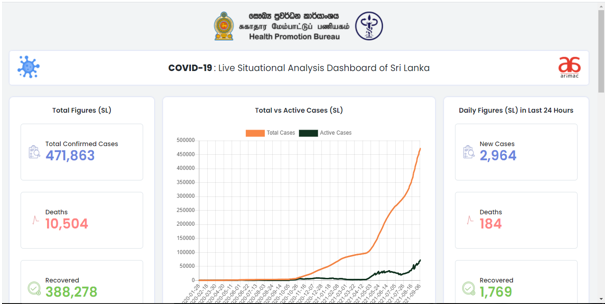
\includegraphics[width=8.4in]{Images/13} \caption{COVID-19 Live Situational Analysis Dashboard of Sri Lanka}\label{fig:unnamed-chunk-20}
\end{figure}

COVID-19 live situation analysis dashboard of Sri Lanka contains total
\& daily figures in Sri Lanka as counts {[}5{]}. Total cases \& active
cases have been visualized by using a line chart. Bar charts have been
used to summarize the daily confirmed cases and recovered cases. As well
fatality rate, recovery rate \& daily investigations using PCR tests \&
rapid antigen tests have been compared by using the bar charts. Doughnut
shape pie chart has been used to summarize the total cases. Blue, green
\& red colors have been applied to active, recovered \& deaths
respectively. This dashboard was also not fitted on a single screen.

\begin{figure}
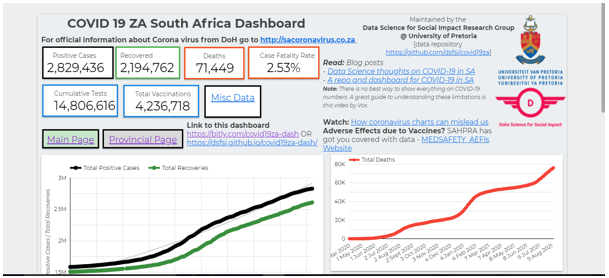
\includegraphics[width=8.46in]{Images/14} \caption{COVID 19 ZA South Africa Dashboard}\label{fig:unnamed-chunk-21}
\end{figure}

Robert Koch-Institute COVID-19 dashboard for German contains interactive
map, line charts \& bar charts as visualization tools of COVID-19 data
{[}12{]}. The dashboard has been fitted on a single screen. This
dashboard format is similar to the John Hopkins dashboard.

\begin{figure}
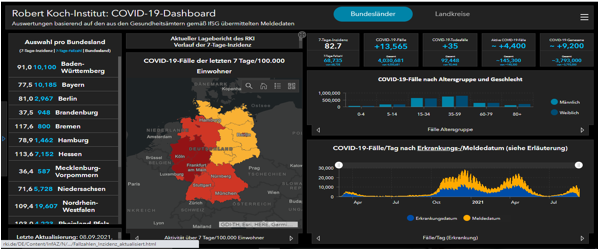
\includegraphics[width=8.33in]{Images/15} \caption{Robert Koch-Institute COVID-19 dashboard for German}\label{fig:unnamed-chunk-22}
\end{figure}

\end{document}
